\subsection{Model}
The model is the most important component of our solution, a badly designed model can imply serious deficulties when implementing new features that are not part of the plans, sometimes we had to redesign the model in order to support new features.

\subsubsection {Generic model}

For designing our model we have taken into account generic programming techniques. We observed that operations like searching for an object was quite repeated amongst different types of objects. 

Our first decision for our model in order to avoid repeated code, was the isolation of the object's attributes from themselves, so we could apply the search operation to a set of attributes indepently from the object type. To this generic set of properties we call data and each object of this type has a reference to the owner, which is a unique identification number.

\begin{figure}[H]
    \centering
    \begin{subfigure}[b]{0.3\textwidth}
    	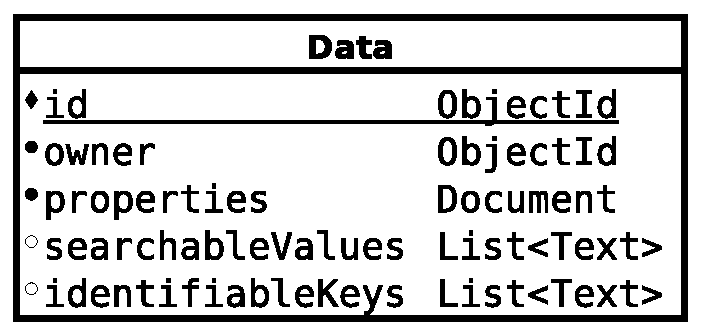
\includegraphics[width=\textwidth]{figures/model_data}
    \end{subfigure}
    \begin{subfigure}[b]{0.35\textwidth}
    	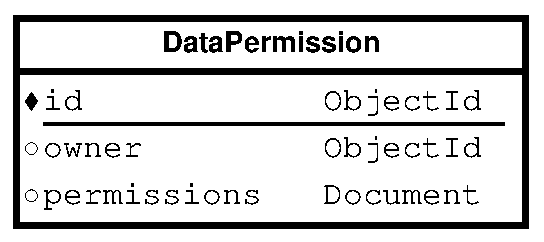
\includegraphics[width=\textwidth]{figures/model_data_permission}
    \end{subfigure}
    \caption{Generic data model}
\end{figure} 

The identication number by itself is not sufficient to identify an object, objects from different types can have the same identification number. In order to solve this problem, when an object is created, its correspondent data must contain the owner's object type. 

When an attribute is created it must be specified if the attribute is searchable, otherwise it could be simple to search for attributes that could reveal sensible information about it. For example if we consider that a user could have a health related attribute, searching by a disease would reveal which users could suffer from a certain disease, the leak of that kind of information could, for instance, change the agreement between users and health insurance companies.

Another important attribute specification is the owner identifiability, which tells us if the attribute identifies the object. This specification let us create abstract authentication services, for example a user can login into our system by providing any attribute that identifies himself, for example the e-mail but others are possible like the username or cellphone number. 

Not less important, attributes can specify aggregations of objects. For example, the user role is an aggregator property that within users it allows the identifaction of each one is administrator. This aggregation specification is independent from the object type, so it's possible to search for the administrative role and return users and groups of users that contains that property.

Our model supports defining read and write permissions for each attribute, for example an attribute can be set to public read access or private write access to a set of entities. Implicitly if an entity can write an attribute it can also read it.




\subsubsection{User model}

The user model is not tied to the user attributes, the information maintained in this model is just used for authentication purposes. Passwords are not stored in plaintext, instead we apply hashing and salting techniques \cite{password} in order to make it harder to decode the password by an attacker. We use \emph{SHA-1} and a random salt per user with 32 characters long.

\begin{figure}[H]
    \centering
    \begin{subfigure}[b]{0.25\textwidth}
    	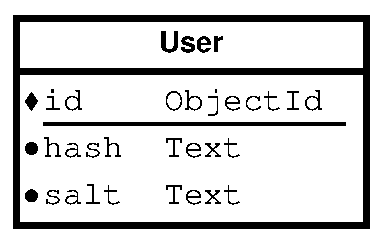
\includegraphics[width=\textwidth]{figures/model_user}
    \end{subfigure}
    \caption{User model}
\end{figure} 

\subsubsection{Relation model}

A relation between two entities $e_1$ and $e_2$ is represented by the pair $e_1\rightarrow e_2$, where $e_1$ is the source and $e_2$ is the target. This relation is said bi-directional if and only if it also exists the relation $e_2\rightarrow e_1$.

\begin{figure}[H]
    \centering
    \begin{subfigure}[b]{0.3\textwidth}
    	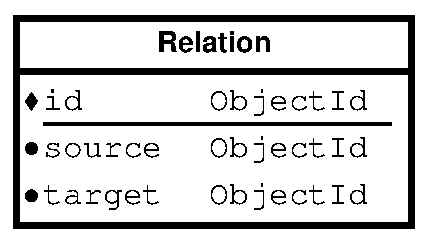
\includegraphics[width=\textwidth]{figures/model_relation}
    \end{subfigure}
    \caption{Relation model}
\end{figure} 

A user can only interact with users that maintain a relationship with him or with users within the same group. In order to validate a relationship, both users must agree on that relationship, by other words it must exist a bi-directional relation between both users.

\subsubsection{Group model}

A group can be public or private. If the group is public then it is visible to all users that mantain a relationship with a member of this group. If the group is private then it is only visible to their members.

\begin{figure}[H]
    \centering
    \begin{subfigure}[b]{0.3\textwidth}
    	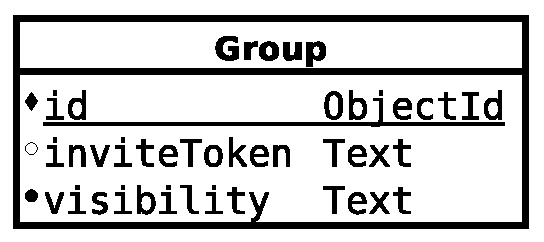
\includegraphics[width=\textwidth]{figures/model_group}
    \end{subfigure}
    \begin{subfigure}[b]{0.3\textwidth}
    	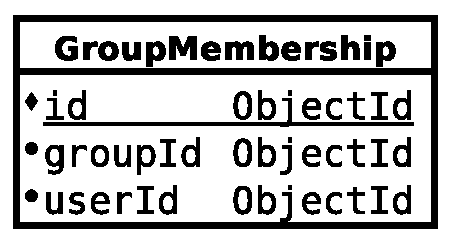
\includegraphics[width=\textwidth]{figures/model_group_membership}
    \end{subfigure}
    \caption{Group model}
\end{figure} 

The group membership is a special case of relation, where the target entity is always a group.

When a group is created, a group membership is automatically assigned by its creator.

Entities that have a membership with a group can create more memberships by sharing an invite token or by specifying new group members.

\subsubsection{Message model}

A message is composed by its content, sequence number, time of creation and source and target identification numbers. The message's target can reference any of object but our application is only covering messages to groups.

\begin{figure}[H]
    \centering
    \begin{subfigure}[b]{0.3\textwidth}
    	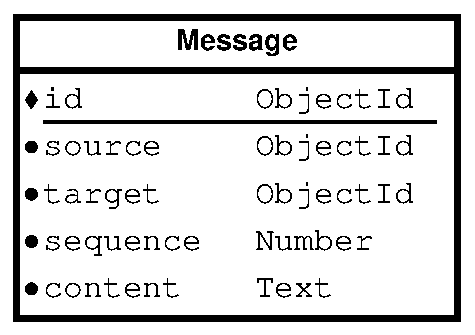
\includegraphics[width=\textwidth]{figures/model_message}
    \end{subfigure}
    \caption{Message model}
\end{figure} 

\subsubsection{Hyper content model}

During a group conversation it is possible to tag points in time for making it easy to access that time either by searching or sharing with other users.

A time tag contains a title, the correspondent group identification number and the time itself.

The hyper content is used to synchronize content among users during a conversation. Every hyper content must have a start and ending time, the correspondent group identification number and the content itself in the form of text.

\begin{figure}[H]
    \centering
    \begin{subfigure}[b]{0.3\textwidth}
    	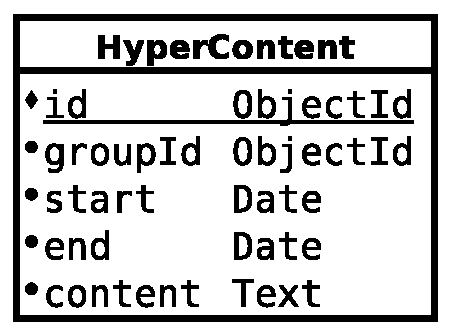
\includegraphics[width=\textwidth]{figures/model_hyper_content}
    \end{subfigure}
    \begin{subfigure}[b]{0.3\textwidth}
    	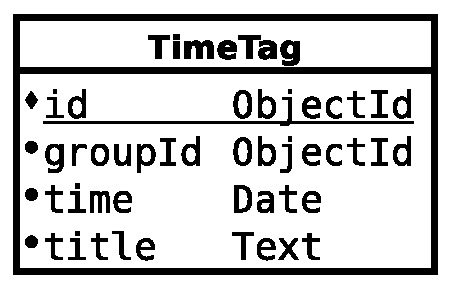
\includegraphics[width=\textwidth]{figures/model_time_tag}
    \end{subfigure}    
    \caption{Hyper content model}
\end{figure} 

\subsubsection{Collaborative Content model}

Within a conversation, users can write documents collaboratively. Each document has a content and a reference to the correspondent group. 

\begin{figure}[H]
    \centering
    \begin{subfigure}[b]{0.3\textwidth}
    	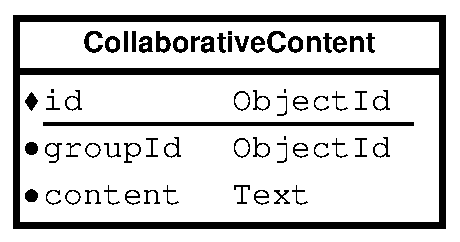
\includegraphics[width=\textwidth]{figures/model_collaborative_content}
    \end{subfigure}
    \caption{Collaborative content model}
\end{figure} 

\subsubsection{Recording model}

During a conversation, users may allow sharing their web cameras, by doing so their video is stored in recording chunks. Each chunk represents an interval of time  $T=[ \,c^{start},c^{end}[ \,$, it contains a reference to a group and a mapping between entity that was recorded and the correspondent video url.

\begin{figure}[H]
    \centering
    \begin{subfigure}[b]{0.3\textwidth}
    	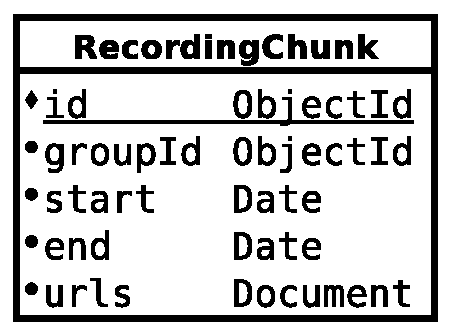
\includegraphics[width=\textwidth]{figures/model_recording_chunk}
    \end{subfigure}
    \begin{subfigure}[b]{0.3\textwidth}
    	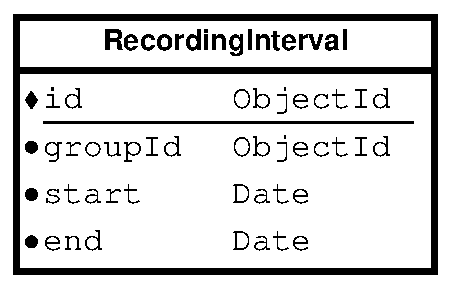
\includegraphics[width=\textwidth]{figures/model_recording_interval}
    \end{subfigure}
    \caption{Recording model}
\end{figure} 

A set of chunks $S=[c_1,c_2,\ldots,c_n]$ is said continuous if $\forall c_i\in S, \exists c_j \in S$ where $j\neq i$ and $c_i^{start} = c_j^{end} \vee c_i^{end} = c_j^{start}$. 

A recording interval represents a continuous set of recording chunks.